% L'option handout permet de supprimer la barre de navigation
\documentclass[handout]{beamer}
\usepackage[utf8]{inputenc}
\usepackage[french]{babel}
\usepackage[T1]{fontenc}
\usepackage{amsmath}
% Pour pouvoir insérer des images
\usepackage{graphicx}
\usepackage{wrapfig}
\graphicspath{images/}
% Gestion des couleurs
\usepackage{color}
\definecolor{red}{RGB}{231, 76, 60}

% Un joli thème flat
\usetheme{Rochester}

% Personnalisation du thème
\usecolortheme[named=red]{structure}
% Numéro de slides dans le footer
\setbeamertemplate{footline}[frame number]
\setbeamertemplate{blocks}[shadow=false]

\newcommand{\intervalleoo}[2]{\mathopen{]}#1\,;#2\mathclose{[}}
\newcommand{\intervalleff}[2]{\mathopen{[}#1\,;#2\mathclose{]}}
\newcommand{\intervalleof}[2]{\mathopen{]}#1\,;#2\mathclose{]}}
\newcommand{\intervallefo}[2]{\mathopen{[}#1\,;#2\mathclose{[}}
\newcommand{\intervalle}[2]{\mathopen{(}#1\,;#2\mathclose{)}}

% ------------------------------------ %
% -- METADONNÉES DU DOCUMENT --------- %
\title{
	Projet OBDE\\
}
\author{
	Équipe MOA : Mickael Billiotte, Anthony Courtin, Quentin Diaferia, Faustine Demiselle\\
	\vspace{10px}
	Équipe MOE : Antoine Augusti, Étienne Batise,  Thibaud Dauce
}
\date{2 juin 2014}

% Générer une page de titre à chaque début de section
\AtBeginSection[]
{
	\begin{frame}[plain]
	\frametitle{Sommaire}
	\tableofcontents[currentsection, hideothersubsections]
	\end{frame}
}

% Début du document
\begin{document}

	% Génération de la page de titre
	\begin{frame}[plain]
		\titlepage
	\end{frame}

	% Génération du sommaire
	\begin{frame}[plain]
		\frametitle{Sommaire}
		\tableofcontents
	\end{frame}

\section{Respect du cahier des charges}

\begin{frame}
	\frametitle{Respect du cahier des charges}

	\begin{figure}
   	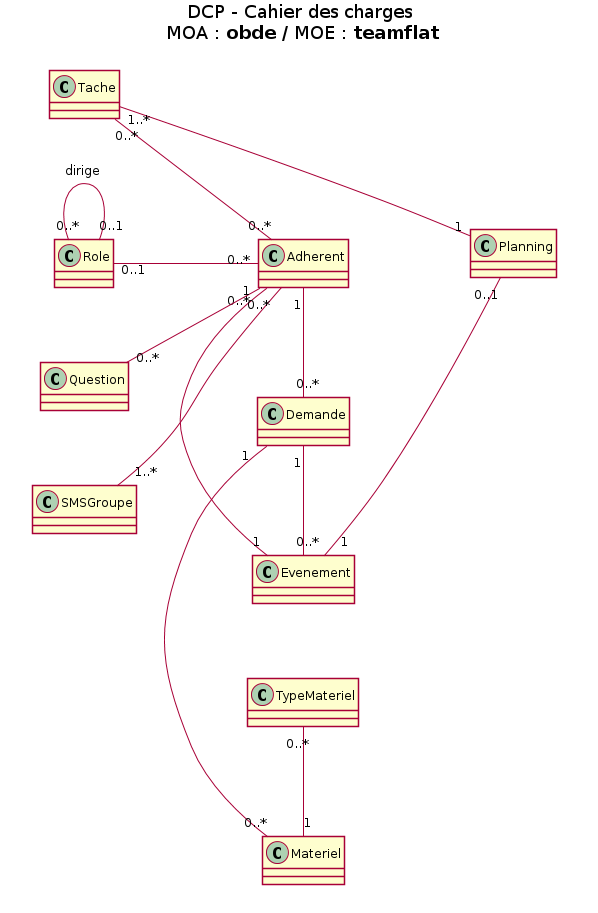
\includegraphics[height= 7.5cm]{images/dcp01.png}
	\end{figure}

\end{frame}

	%
	%% Adhérents
	%
	\subsection{Adhérents}
	\begin{frame}
		\frametitle{Adhérents}

		\begin{itemize}
			\item Gestion des questions
			\item SMS groupés
			\item Tâches
			\item Rôles
			\item Demande
		\end{itemize}

		\begin{exampleblock}{Liste des exigences qualifiées ID 13}
			Un système de foire aux questions sera disponible.
		\end{exampleblock}
	\end{frame}

	%
	%% Rôles
	%
	\subsection{Rôles}
	\begin{frame}
		\frametitle{Rôles}

		\begin{itemize}
			\item Gestion des rôles multiples
			\item Gestion de la hierarchie entre les différents rôles
		\end{itemize}

		\begin{exampleblock}{Liste des exigences qualifiées ID 4}
			L'application sera capable de gérer une hierarchie entre les utilisateurs : membres du bureau, reponsables de pôles, membre de l'équipe.
		\end{exampleblock}
	\end{frame}

	%
	%% Évènements
	%
	\subsection{Évènements}
	\begin{frame}
		\frametitle{Évènements}

		\begin{itemize}
			\item Possibilité d'ajouter un planning
			\item Gestion des tâches
			\item Gestion des demandes
		\end{itemize}

		\begin{exampleblock}{Cahier des charges - Partie 3.3.2}
			... les membres de l'équipe BDE sont notifiés sur l'application de la création d'un nouvel événement et peuvent s'inscrire sur un planning.
		\end{exampleblock}
	\end{frame}

	%
	%% Demandes
	%
	\subsection{Demandes}
	\begin{frame}
		\frametitle{Demandes}

		\begin{itemize}
			\item Liées à un événement
			\item Possiblité de gérer le matériel
		\end{itemize}

		\begin{exampleblock}{Liste des exigences qualifiées  ID 14}
			... l'application pourra accéder au matériel disponible pour organiser un évément.
		\end{exampleblock}
	\end{frame}

	% //////////////////////////////// %
	% /// Présentation /////////////// %
	% \section{Présentation}

	% 	%
	% 	%% Origine
	% 	%
	% 	\subsection{Origine}
	% 	\begin{frame}
	% 		\frametitle{Origine}

	% 		Création :
	% 		\begin{itemize}
	% 			\item Proposé par Quenouille dans les années 50 pour le calcul de biais
	% 			\item Repris par Tuckey pour l'estimation de la variance, tester une hypothèse ou établir un intervalle de confiance
	% 		\end{itemize}


	% 		\vspace{20px}

	% 		\begin{exampleblock}{Que signifie Jackknife ?}
	% 			Jackknife signifie en anglais couteau suisse. Cet outil a été nommé ainsi car, comme l'objet, c'est un outil pratique et rapide pouvant remplacer des outils plus sophistiqués et compliqués.
	% 		\end{exampleblock}
	% 	\end{frame}

% Fin du document
\end{document}
